\documentclass{article}
\usepackage[utf8x]{inputenc}
\usepackage{tikz}
\usepackage{lscape}
\usepackage{pdflscape}
\usepackage{pdfpages}
\usepackage{amstext}
\usepackage[scale=0.75,top=1cm]{geometry}
\begin{document}
\begin{titlepage}
    \begin{center}
        \vspace*{1cm}

        \Huge
        \textbf{PDL: Práctica Procesador}
        
        \vspace{0.5cm}
        \large
        Segunda Entrega: \\
        Analizador Sintactíco
        \vspace{3cm}
       
        \textbf{
            Serrano,Arrese Francisco Javier\\
            Cañibano,Lopez Alberto\\
            Vallejo,Collados Jesús
            }
            
        \vspace{8cm}
    
        \large
        Grupo 14 \\
        Procesadores de Lenguajes\\
        Universidad Politécnica de Madrid\\
        Curso 2020-2021
        
    \end{center}
\end{titlepage}
\newpage
Gramática Analizador Sintáctico
\begin{verbatim}
NoTerminales = { E R U V S L Q X B T F H A K C P V1 S1 E1 R1 U1 }
Terminales = { && == != + - ID ( ) ENT CAD TRUE FALSE ! ++ ALERT INPUT 
               RETURN DO WHILE , ; = NUMBER BOOLEAN STRING FUNCTION LET { } IF }
Axioma = P
Producciones = {
E -> R E1
E1 -> && R E1
E1 -> lambda
R -> U R1
R1 -> == U R1
R1 -> != U R1
R1 -> lambda
U -> V U1
U1 -> + V U1
U1 -> - V U1
U1 -> lambda
V -> ID V1
V -> ( E ) 
V -> ENT 
V -> CAD 
V -> TRUE 
V -> FALSE 
V -> ! ID
V1 -> ( L )
V1 -> ++
V1 -> lambda
S -> ID S1
S -> ALERT ( E ) ;
S -> INPUT ( ID ) ;
S -> RETURN X ;
S1 -> = E ;
S1 -> ( L ) ;
L -> E Q 
L -> lambda
Q -> , E Q 
Q -> lambda
X -> E 
X -> lambda
B -> IF ( E ) S 
B -> LET T ID ;
B -> S
B -> DO { C } WHILE ( E ) ;
T -> NUMBER 
T -> BOOLEAN 
T -> STRING
F -> FUNCTION H ID ( A ) { C }
H -> T 
H -> lambda
A -> T ID K 
A -> lambda
K -> , T ID K 
K -> lambda
C -> B C 
C -> lambda
P -> B P 
P -> F P
P -> lambda
}
\end{verbatim}


Tabla First Follow
\begin{verbatim}

            First                                           Follow
A       BOOLEAN NUMBER STRING lambda                    .. )
T       BOOLEAN NUMBER STRING                           ..  
B       ALERT DO ID IF INPUT LET RETURN                 ..
S       ALERT ID INPUT RETURN                           .. 
S1      ( =                                             .. 
C       ALERT DO ID IF INPUT LET RETURN lambda          .. }
E       ! ( CAD ENT FALSE ID TRUE                       .. ) , ; 
E1      && lambda                                       .. ) , ;
V       ! ( CAD ENT FALSE ID TRUE                       .. != && ) + , - ; ==
V1      ( ++ lambda                                     .. != && ) + , - ; ==
U       ! ( CAD ENT FALSE ID TRUE                       .. != && ) , ; ==
U1      + - lambda                                      .. != && ) , ; ==
R       ! ( CAD ENT FALSE ID TRUE                       .. && ) , ;
R1      != == lambda                                    .. && ) , ;
Q       , lambda                                        .. )
L       ! ( CAD ENT FALSE ID TRUE lambda                .. )
X       ! ( CAD ENT FALSE ID TRUE lambda                .. ;
F       FUNCTION                                        .. 
H       BOOLEAN NUMBER STRING lambda                    .. ID
K       , lambda                                        .. )
P       ALERT DO FUNCTION ID IF INPUT LET RETURN lambda .. $ (final de cadena)
\end{verbatim}

\newpage
Análisis de las intersecciones (@ es el símbolo de intersección)
\begin{verbatim}

Para P:
    -B: {ALERT DO ID IF INPUT LET RETURN}
    -F: {FUNCTION}
    -lambda: lambda
    Interseccion: 
        -First(BP) @ First(FP) @ First(lambda) = Vacio
        -First(BP) @ Follow(P) @ First(FP) = Vacio
        
Para C:
    -B:{ALERT DO ID IF INPUT LET RETURN}
    -lambda: lambda
        -First(BC) @ First(lambda) = Vacio
        -First(BC) @ Follow(C) = Vacio

Para K:
    
        -First(,T ID K) @ First(lambda) = Vacio
        -First(,T ID K) @ Follow(A) = Vacio

Para H:
    -T: {BOOLEAN NUMBER STRING}
    -lambda: lambda
        -First(T) @ First(lambda) = Vacio        
        -First(T) @ Follow(H) = Vacio

Para F:

Para T:
    
        -First(NUMBER) @ First(BOOLEAN) @ First(STRING) = Vacio
        
Para B:
    -S: {ID ALERT INPUT RETURN}
        -First(IF ( E ) S) @ First(LET T ID) @ First(S) @ First(DO { C } WHILE ( E );) = Vacio

Para X:
    -E: {! ( CAD ENT FALSE ID TRUE}
    -lambda: lambda
        -First(E) @ First(lambda) = Vacio
        -First(E) @ Follow(X) = Vacio

Para Q: 
    -lambda: lambda
        -First(, E Q) @ First(lambda) = Vacio
        -First(, E Q) @ Follow(Q) = Vacio

      
Para L:
    -E:{! ( CAD ENT FALSE ID TRUE}
    -lambda: lambda
        -First(E Q) @ First(lambda) = Vacio 
        -First(E Q) @ Follow(L) = Vacio  

Para S1: 
        -First(= E ;) @ First(( L ) ;) = Vacio

Para S:
        -First(RETURN X ;) @ First(INPUT ( ID ) ;) @ First(ALERT ( E ) ;) @ First(ID S1) = Vacio

Para V1: 
    -lambda: lambda
        -First(( L )) @ First(++) @ First(lambda) = Vacio
        -First(( L )) @ First(++) @ Follow(V1) = Vacio

Para V: 
        -First(ID V1) @ First(( E )) @ First(ENT) @ First(CAD) @ First(TRUE) @ First(FALSE) @ First(! ID) = Vacio

Para U1: 
    - lambda: lambda
        -First(+ V U1) @ First(- V U1) @ First(lambda) = Vacio
        -First(+ V U1) @ First(- V U1) @ Follow(U1) = Vacio

Para U:

Para E:

Para E1:
    -lambda: lambda
        -First(&& R E1) @ First(lambda) = Vacio
        -First(&& R E1) @ Follow(E1) = Vacio
Para R:

Para R1:
    -lambda: lambda
        -First(== U R1)@ First(!= U R1)@ First(!= U R1) = Vacio
        -First(== U R1)@ First(!= U R1)@ Follow(R1) = Vacio
\end{verbatim}
Tabla LL(1)
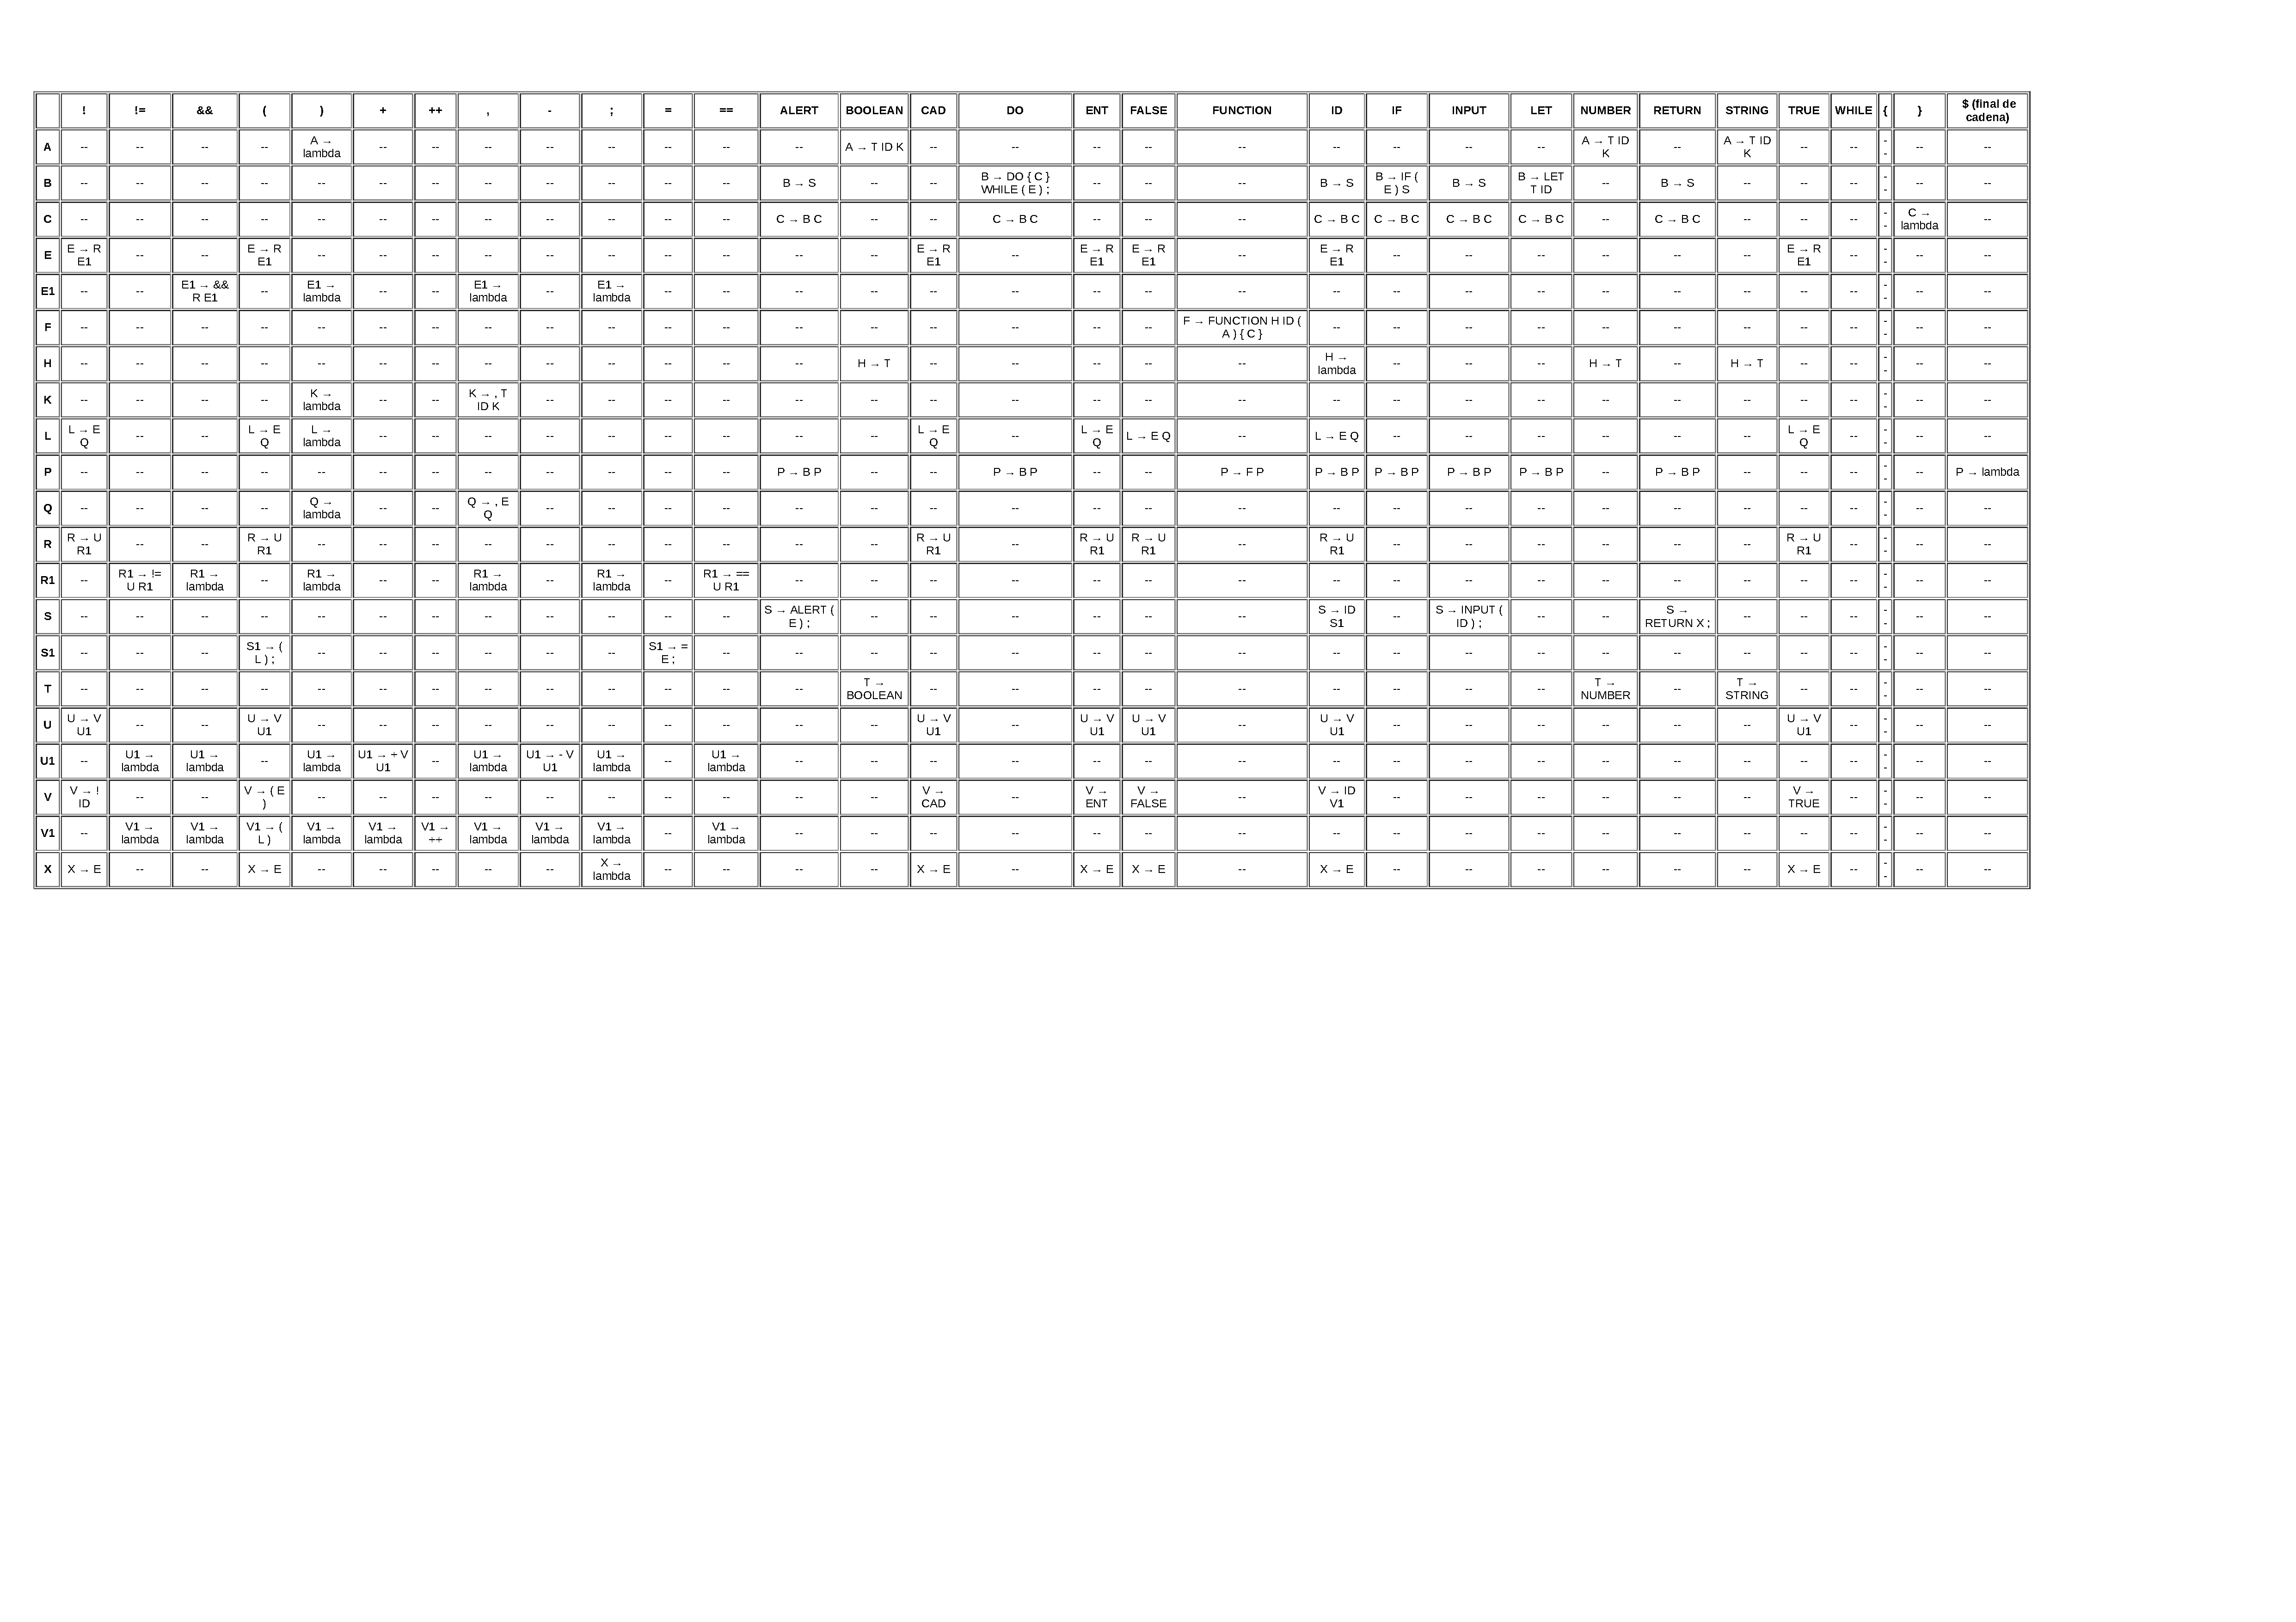
\includepdf{TABLA.pdf}
\newpage
\vspace{5cm}
Por tanto podemos concluir que la gramática al no tener recursividad por la izquierda, estar factorizada y ser LL(1), es una gramática correcta para un
analizador sintáctico, del tipo descendente recursivo.
\vspace{3cm}

Prueba 1 correcta
\begin{verbatim}
---------------------------------
---------- código ---------------
---------------------------------
let number a;
let number b;
let number int;
alert ('Introduce el primer operando');
input (a);
alert ('Introduce el segundo operando');
input (b);
function number operacion (number num1, number num2)
{
	let number res;
	res = num1-num2;
	return res;
}
int = operacion (a, b);
alert (int);
---------------------------------
---------- tokens ---------------
---------------------------------
<reservedWord,let>
<reservedWord,number>
<ID,1>
<separator,semicolon>
<reservedWord,let>
<reservedWord,number>
<ID,2>
<separator,semicolon>
<reservedWord,let>
<reservedWord,number>
<ID,3>
<separator,semicolon>
<reservedWord,alert>
<separator,openPar>
<chain,"Introduce el primer operando">
<separator,closePar>
<separator,semicolon>
<reservedWord,input>
<separator,openPar>
<ID,3>
<separator,closePar>
<separator,semicolon>
<reservedWord,alert>
<separator,openPar>
<chain,"Introduce el segundo operando">
<separator,closePar>
<separator,semicolon>
<reservedWord,input>
<separator,openPar>
<ID,3>
<separator,closePar>
<separator,semicolon>
<reservedWord,function>
<reservedWord,number>
<ID,4>
<separator,openPar>
<reservedWord,number>
<ID,5>
<separator,colon>
<reservedWord,number>
<ID,6>
<separator,closePar>
<separator,openBraq>
<reservedWord,let>
<reservedWord,number>
<ID,7>
<separator,semicolon>
<ID,7>
<asigOp,equal>
<ID,7>
<aritOp,minus>
<ID,7>
<separator,semicolon>
<reservedWord,return>
<ID,7>
<separator,semicolon>
<separator,closeBraq>
<ID,7>
<asigOp,equal>
<ID,7>
<separator,openPar>
<ID,7>
<separator,colon>
<ID,7>
<separator,closePar>
<separator,semicolon>
<reservedWord,alert>
<separator,openPar>
<ID,7>
<separator,closePar>
<separator,semicolon>
---------------------------------
------------ ts -----------------
---------------------------------
Contenido Tabla Simbolos # 0 :
* LEXEMA : 'a'
  ATRIBUTOS :
* LEXEMA : 'b'
  ATRIBUTOS :
* LEXEMA : 'int'
  ATRIBUTOS :
* LEXEMA : 'operacion'
  ATRIBUTOS :
* LEXEMA : 'num1'
  ATRIBUTOS :
* LEXEMA : 'num2'
  ATRIBUTOS :
* LEXEMA : 'res'
  ATRIBUTOS :
---------------------------------
----------- parse ---------------
---------------------------------
Descendente 50 35 38 50 35 38 50 35 38 50 36 23 1 4 8 15 11 7 3 50 36 24 50 36 23 1 4 8 15 11 7 3 
50 36 24 51 41 42 38 44 38 46 38 47 48 35 38 48 36 22 26 1 4 8 12 21 10 12 21 11 7 3 48 36 25 32 1 
4 8 12 21 11 7 3 49 50 36 22 26 1 4 8 12 19 28 1 4 8 12 21 11 7 3 30 1 4 8 12 21 11 7 3 31 11 7 3 50 
36 23 1 4 8 12 21 11 7 3 52
---------------------------------
---------- errors ---------------
---------------------------------
\end{verbatim}
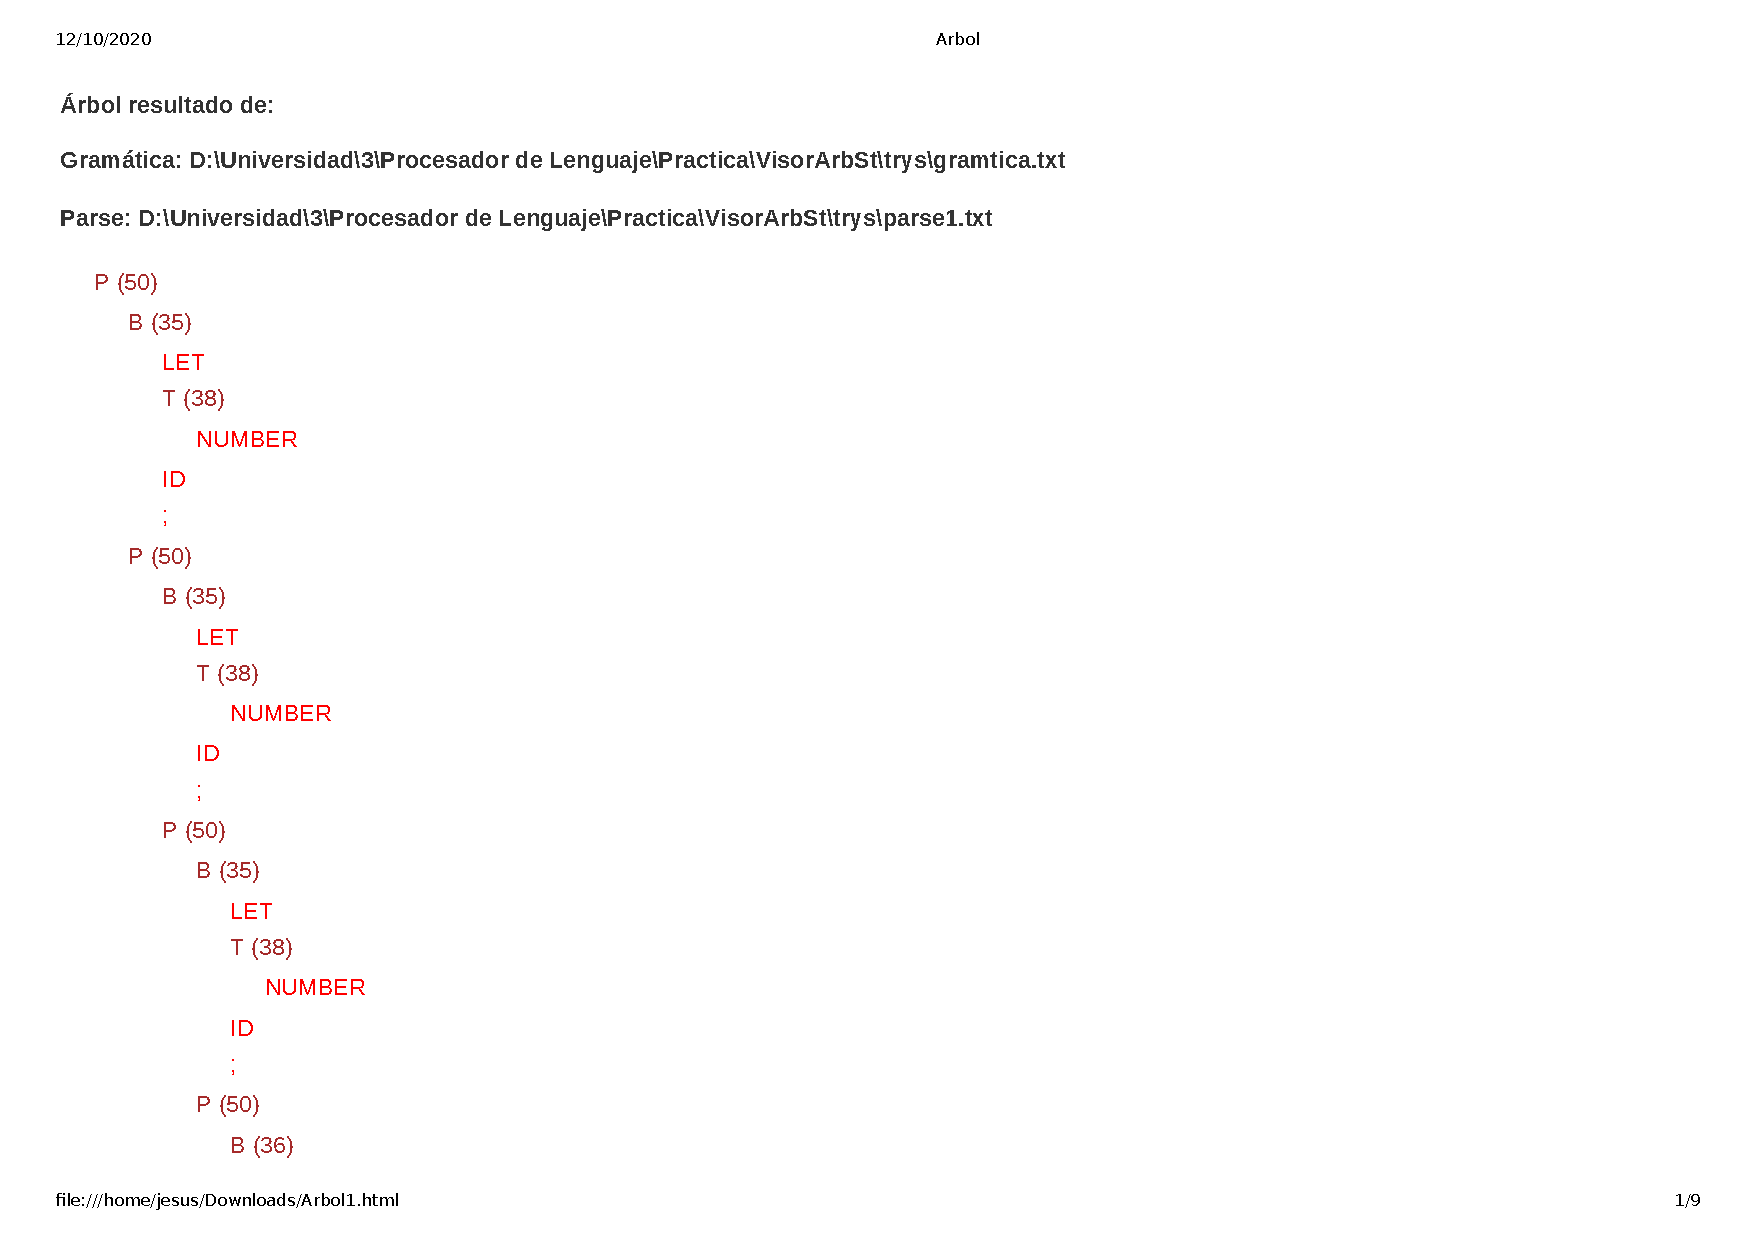
\includepdf[pages={1-},scale=1]{Arbol1.pdf}
\newpage
Prueba 2 correcta
\begin{verbatim}
---------------------------------
---------- código ---------------
---------------------------------
let number a;
let number b;
let boolean bbb;
a = 3;
b = a;
let boolean c;
c = a == b;
if (c) b = 3333;
a = a + b;
alert (a);
alert(b);
---------------------------------
---------- tokens ---------------
---------------------------------
<reservedWord,let>
<reservedWord,number>
<ID,1>
<separator,semicolon>
<reservedWord,let>
<reservedWord,number>
<ID,2>
<separator,semicolon>
<reservedWord,let>
<reservedWord,boolean>
<ID,3>
<separator,semicolon>
<ID,3>
<asigOp,equal>
<wholeConst,3>
<separator,semicolon>
<ID,3>
<asigOp,equal>
<ID,3>
<separator,semicolon>
<reservedWord,let>
<reservedWord,boolean>
<ID,4>
<separator,semicolon>
<ID,4>
<asigOp,equal>
<ID,4>
<relOp,equals>
<ID,4>
<separator,semicolon>
<reservedWord,if>
<separator,openPar>
<ID,4>
<separator,closePar>
<ID,4>
<asigOp,equal>
<wholeConst,3333>
<separator,semicolon>
<ID,4>
<asigOp,equal>
<ID,4>
<aritOp,plus>
<ID,4>
<separator,semicolon>
<reservedWord,alert>
<separator,openPar>
<ID,4>
<separator,closePar>
<separator,semicolon>
<reservedWord,alert>
<separator,openPar>
<ID,4>
<separator,closePar>
<separator,semicolon>
---------------------------------
------------ ts -----------------
---------------------------------
Contenido Tabla Simbolos # 0 :
* LEXEMA : 'a'
  ATRIBUTOS :
* LEXEMA : 'b'
  ATRIBUTOS :
* LEXEMA : 'bbb'
  ATRIBUTOS :
* LEXEMA : 'c'
  ATRIBUTOS :
---------------------------------
----------- parse ---------------
---------------------------------
Descendente 50 35 38 50 35 38 50 35 39 50 36 22 26 1 4 8 14 11 7 3 50 36 22 26 1 4 8 12 21 11 7 3 50 
35 39 50 36 22 26 1 4 8 12 21 11 5 8 12 21 11 7 3 50 34 1 4 8 12 21 11 7 3 22 26 1 4 8 14 11 7 3 50 
36 22 26 1 4 8 12 21 9 12 21 11 7 3 50 36 23 1 4 8 12 21 11 7 3 50 36 23 1 4 8 12 21 11 7 3 52
---------------------------------
---------- errors ---------------
---------------------------------
\end{verbatim}
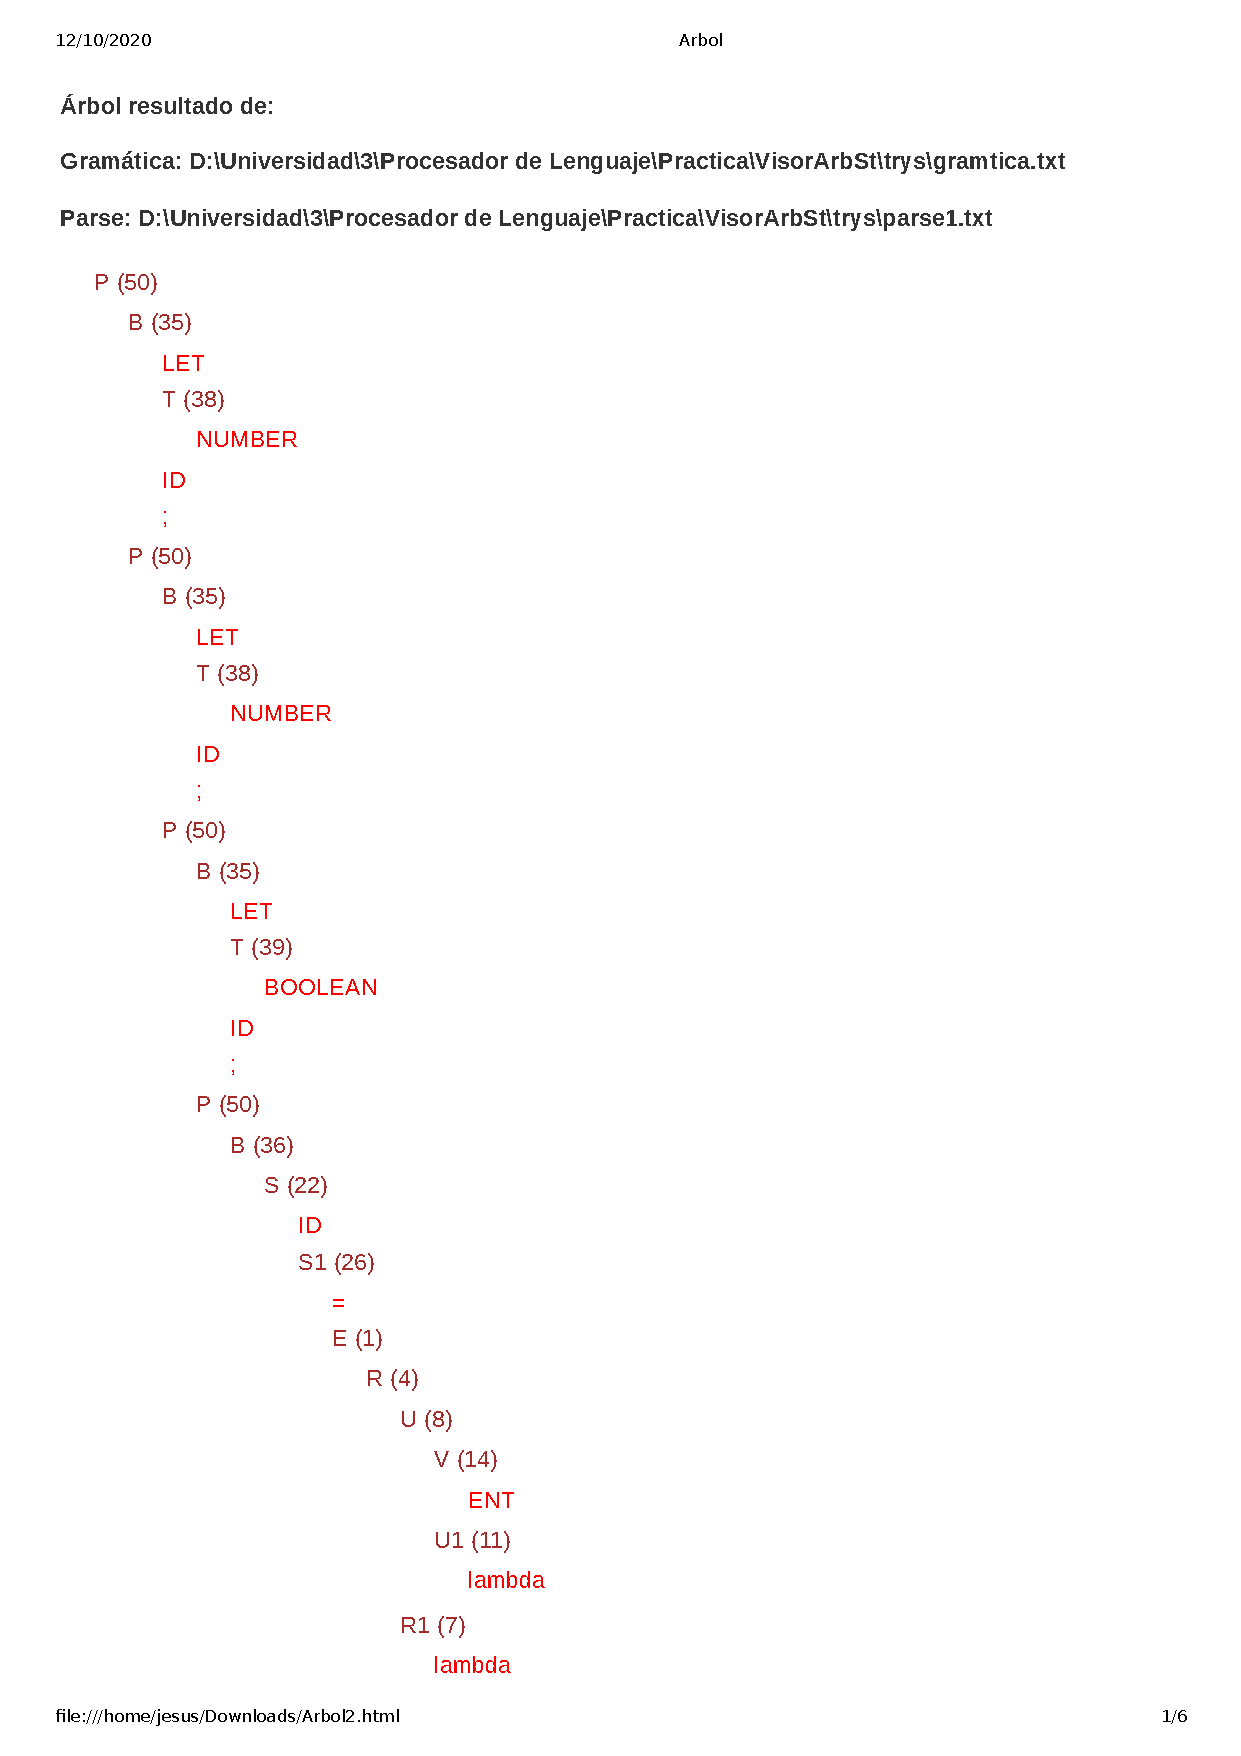
\includepdf[pages={1-},scale=1]{Arbol2.pdf}
\newpage
Prueba 3 correcta
\begin{verbatim}
---------------------------------
---------- código ---------------
---------------------------------
let number x;
let number z;
let boolean b;

alert ('PdL');
input (esto_es_un_nombre_de_variable_global_de_tipo_entero);
input (z);
alert (z);
x=z;
alert (z-1);
b=b&&b;if (b)
x =
  x + 6
    - z
    + 1
    - (2
    - y
    + 6);
---------------------------------
---------- tokens ---------------
---------------------------------
<reservedWord,let>
<reservedWord,number>
<ID,1>
<separator,semicolon>
<reservedWord,let>
<reservedWord,number>
<ID,2>
<separator,semicolon>
<reservedWord,let>
<reservedWord,boolean>
<ID,3>
<separator,semicolon>
<reservedWord,alert>
<separator,openPar>
<chain,"PdL">
<separator,closePar>
<separator,semicolon>
<reservedWord,input>
<separator,openPar>
<ID,4>
<separator,closePar>
<separator,semicolon>
<reservedWord,input>
<separator,openPar>
<ID,4>
<separator,closePar>
<separator,semicolon>
<reservedWord,alert>
<separator,openPar>
<ID,4>
<separator,closePar>
<separator,semicolon>
<ID,4>
<asigOp,equal>
<ID,4>
<separator,semicolon>
<reservedWord,alert>
<separator,openPar>
<ID,4>
<aritOp,minus>
<wholeConst,1>
<separator,closePar>
<separator,semicolon>
<ID,4>
<asigOp,equal>
<ID,4>
<logOp,and>
<ID,4>
<separator,semicolon>
<reservedWord,if>
<separator,openPar>
<ID,4>
<separator,closePar>
<ID,4>
<asigOp,equal>
<ID,4>
<aritOp,plus>
<wholeConst,6>
<aritOp,minus>
<ID,4>
<aritOp,plus>
<wholeConst,1>
<aritOp,minus>
<separator,openPar>
<wholeConst,2>
<aritOp,minus>
<ID,5>
<aritOp,plus>
<wholeConst,6>
<separator,closePar>
<separator,semicolon>
---------------------------------
------------ ts -----------------
---------------------------------
Contenido Tabla Simbolos # 0 :
* LEXEMA : 'x'
  ATRIBUTOS :
* LEXEMA : 'z'
  ATRIBUTOS :
* LEXEMA : 'b'
  ATRIBUTOS :
* LEXEMA : 'esto_es_un_nombre_de_variable_global_de_tipo_entero'
  ATRIBUTOS :
* LEXEMA : 'y'
  ATRIBUTOS :
---------------------------------
----------- parse ---------------
---------------------------------
Descendente 50 35 38 50 35 38 50 35 39 50 36 23 1 4 8 15 11 7 3 50 36 24 50 36 24 50 36 
23 1 4 8 12 21 11 7 3 50 36 22 26 1 4 8 12 21 11 7 3 50 36 23 1 4 8 12 21 10 14 11 7 3 
50 36 22 26 1 4 8 12 21 11 7 2 4 8 12 21 11 7 3 50 34 1 4 8 12 21 11 7 3 22 26 1 4 8 12 
21 9 14 10 12 21 9 14 10 13 1 4 8 14 10 12 21 9 14 11 7 3 11 7 3 52
---------------------------------
---------- errors ---------------
---------------------------------
\end{verbatim}
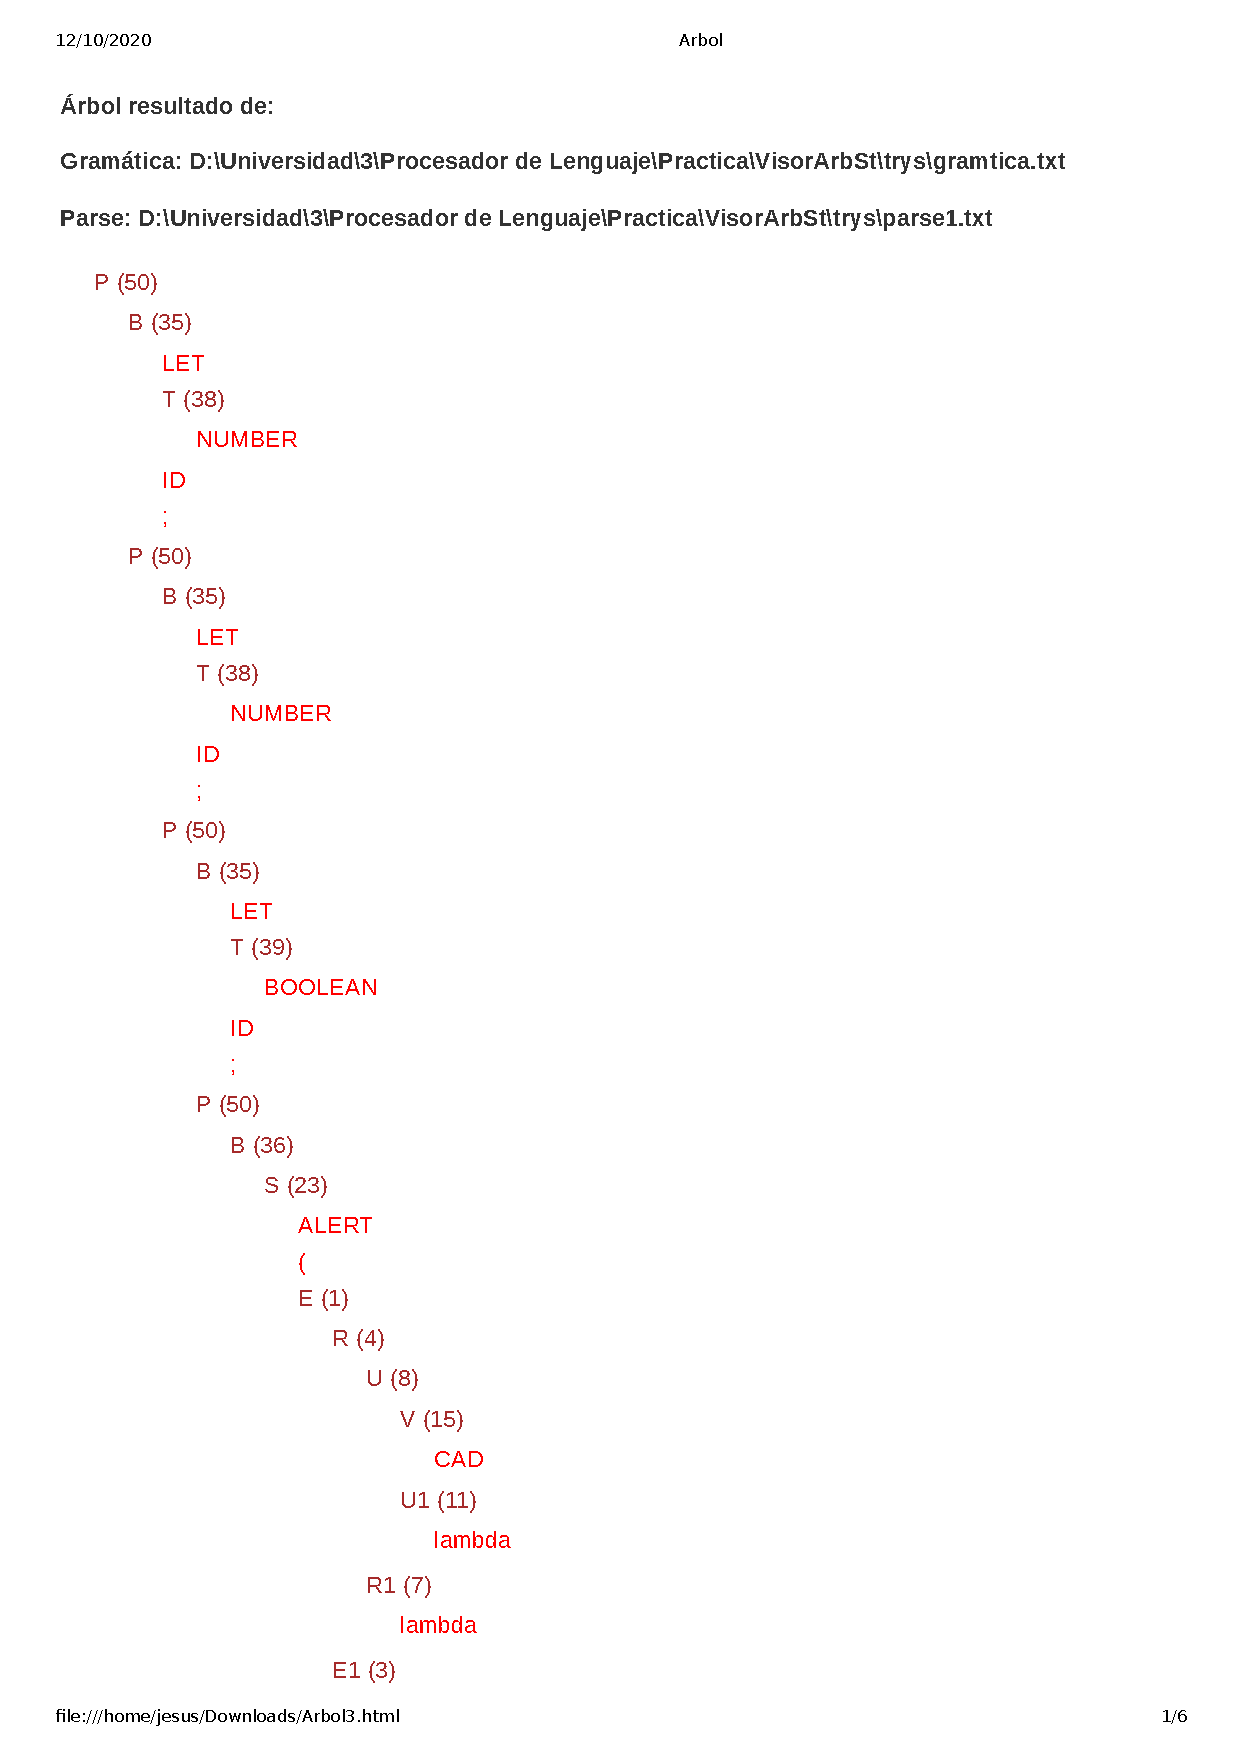
\includepdf[pages={1-},scale=1]{Arbol3.pdf}
\newpage
Prueba 4 incorrecta
\begin{verbatim}
---------------------------------
---------- codigo ---------------
---------------------------------
let number x;
let number z;
let boolean b;

alert ('PdL');
input (esto_es_un_nombre_de_variable_global_de_tipo_entero);
input (z);
aler;
x=z;
alert (z-1);
b=b&&b;if (b)
x =
  x + 6
    - z
    + 1
    - (2
    - y
    + 6);
---------------------------------
---------- tokens ---------------
---------------------------------
<reservedWord,let>
<reservedWord,number>
<ID,1>
<separator,semicolon>
<reservedWord,let>
<reservedWord,number>
<ID,2>
<separator,semicolon>
<reservedWord,let>
<reservedWord,boolean>
<ID,3>
<separator,semicolon>
<reservedWord,alert>
<separator,openPar>
<chain,"PdL">
<separator,closePar>
<separator,semicolon>
<reservedWord,input>
<separator,openPar>
<ID,4>
<separator,closePar>
<separator,semicolon>
<reservedWord,input>
<separator,openPar>
<ID,4>
<separator,closePar>
<separator,semicolon>
<ID,5>
<separator,semicolon>
<ID,5>
<asigOp,equal>
<ID,5>
<separator,semicolon>
<reservedWord,alert>
<separator,openPar>
<ID,5>
<aritOp,minus>
<wholeConst,1>
<separator,closePar>
<separator,semicolon>
<ID,5>
<asigOp,equal>
<ID,5>
<logOp,and>
<ID,5>
<separator,semicolon>
<reservedWord,if>
<separator,openPar>
<ID,5>
<separator,closePar>
<ID,5>
<asigOp,equal>
<ID,5>
<aritOp,plus>
<wholeConst,6>
<aritOp,minus>
<ID,5>
<aritOp,plus>
<wholeConst,1>
<aritOp,minus>
<separator,openPar>
<wholeConst,2>
<aritOp,minus>
<ID,6>
<aritOp,plus>
<wholeConst,6>
<separator,closePar>
<separator,semicolon>
---------------------------------
------------ ts -----------------
---------------------------------
Contenido Tabla Simbolos # 0 :
* LEXEMA : 'x'
  ATRIBUTOS :
* LEXEMA : 'z'
  ATRIBUTOS :
* LEXEMA : 'b'
  ATRIBUTOS :
* LEXEMA : 'esto_es_un_nombre_de_variable_global_de_tipo_entero'
  ATRIBUTOS :
* LEXEMA : 'aler'
  ATRIBUTOS :
* LEXEMA : 'y'
  ATRIBUTOS :
---------------------------------
----------- parse ---------------
---------------------------------

---------------------------------
---------- errors ---------------
---------------------------------
ErrorSintactico: Error en regla S1
\end{verbatim}

Prueba 5 incorrecta
\begin{verbatim}
---------------------------------
---------- codigo ---------------
---------------------------------
let number a;
let number b;
let number int;
alert ('Introduce el primer operando');
input (a);
('Introduce el segundo operando');
input (b);
function number operacion (number num1, number num2)
{
	let number res;
	res = num1-num2;
	return res;
}
int = operacion (a, b);
alert (int);
---------------------------------
---------- tokens ---------------
---------------------------------
<reservedWord,let>
<reservedWord,number>
<ID,1>
<separator,semicolon>
<reservedWord,let>
<reservedWord,number>
<ID,2>
<separator,semicolon>
<reservedWord,let>
<reservedWord,number>
<ID,3>
<separator,semicolon>
<reservedWord,alert>
<separator,openPar>
<chain,"Introduce el primer operando">
<separator,closePar>
<separator,semicolon>
<reservedWord,input>
<separator,openPar>
<ID,3>
<separator,closePar>
<separator,semicolon>
<separator,openPar>
<chain,"Introduce el segundo operando">
<separator,closePar>
<separator,semicolon>
<reservedWord,input>
<separator,openPar>
<ID,3>
<separator,closePar>
<separator,semicolon>
<reservedWord,function>
<reservedWord,number>
<ID,4>
<separator,openPar>
<reservedWord,number>
<ID,5>
<separator,colon>
<reservedWord,number>
<ID,6>
<separator,closePar>
<separator,openBraq>
<reservedWord,let>
<reservedWord,number>
<ID,7>
<separator,semicolon>
<ID,7>
<asigOp,equal>
<ID,7>
<aritOp,minus>
<ID,7>
<separator,semicolon>
<reservedWord,return>
<ID,7>
<separator,semicolon>
<separator,closeBraq>
<ID,7>
<asigOp,equal>
<ID,7>
<separator,openPar>
<ID,7>
<separator,colon>
<ID,7>
<separator,closePar>
<separator,semicolon>
<reservedWord,alert>
<separator,openPar>
<ID,7>
<separator,closePar>
<separator,semicolon>
---------------------------------
------------ ts -----------------
---------------------------------
Contenido Tabla Simbolos # 0 :
* LEXEMA : 'a'
  ATRIBUTOS :
* LEXEMA : 'b'
  ATRIBUTOS :
* LEXEMA : 'int'
  ATRIBUTOS :
* LEXEMA : 'operacion'
  ATRIBUTOS :
* LEXEMA : 'num1'
  ATRIBUTOS :
* LEXEMA : 'num2'
  ATRIBUTOS :
* LEXEMA : 'res'
  ATRIBUTOS :
---------------------------------
----------- parse ---------------
---------------------------------

---------------------------------
---------- errors ---------------
---------------------------------
ErrorSintactico: Error en regla P
\end{verbatim}

Prueba 6 incorrecta
\begin{verbatim}
---------------------------------
---------- codigo ---------------
---------------------------------
let number a;
let number b;
let boolean bbb;
a = 3;
b = a;
let boolean c;
c = a == b;
if (c) b = 3333
a = a + b;
alert (a);
alert(b);
---------------------------------
---------- tokens ---------------
---------------------------------
<reservedWord,let>
<reservedWord,number>
<ID,1>
<separator,semicolon>
<reservedWord,let>
<reservedWord,number>
<ID,2>
<separator,semicolon>
<reservedWord,let>
<reservedWord,boolean>
<ID,3>
<separator,semicolon>
<ID,3>
<asigOp,equal>
<wholeConst,3>
<separator,semicolon>
<ID,3>
<asigOp,equal>
<ID,3>
<separator,semicolon>
<reservedWord,let>
<reservedWord,boolean>
<ID,4>
<separator,semicolon>
<ID,4>
<asigOp,equal>
<ID,4>
<relOp,equals>
<ID,4>
<separator,semicolon>
<reservedWord,if>
<separator,openPar>
<ID,4>
<separator,closePar>
<ID,4>
<asigOp,equal>
<wholeConst,3333>
<ID,4>
<asigOp,equal>
<ID,4>
<aritOp,plus>
<ID,4>
<separator,semicolon>
<reservedWord,alert>
<separator,openPar>
<ID,4>
<separator,closePar>
<separator,semicolon>
<reservedWord,alert>
<separator,openPar>
<ID,4>
<separator,closePar>
<separator,semicolon>
---------------------------------
------------ ts -----------------
---------------------------------
Contenido Tabla Simbolos # 0 :
* LEXEMA : 'a'
  ATRIBUTOS :
* LEXEMA : 'b'
  ATRIBUTOS :
* LEXEMA : 'bbb'
  ATRIBUTOS :
* LEXEMA : 'c'
  ATRIBUTOS :
---------------------------------
----------- parse ---------------
---------------------------------

---------------------------------
---------- errors ---------------
---------------------------------
ErrorSintactico: Error en regla R2
\end{verbatim}

\end{document}

    }